\documentclass{spektraklet}

\begin{document}

%----------------------------------------------------------------------
%	arguments:
%		#1	publication number (eg. 1/2015, 2/2015, 3/2015 etc.),
%			the year is filled in programatically.
%
%		#2	the width of the cover image
%
%		#3	the path to the cover image
%
%		#4	optional argument with offsets for the cover image
%----------------------------------------------------------------------
\titlepage{Gulisnummer}{\paperwidth}{bilder/parm.jpg}[0, -2cm]
%\titlepage{1}{0.75\linewidth}{images/dog.jpg}



%----------------------------------------------------------------------
%	There are a couple of fields in the content page that is changable,
%	and some of them are mandatory. The default values are defined in
%	the 'spektraklet.cls' file.
%
%	Mandator:
%		\ChiefEditor{name}
%		\ManagingEditor{name}
%		\Editors{name1\\name2\\name3}	the last name shouldn't be followed by a \\
%
%	Optional:							Default value:
%		\PublicationInformation[text]		Àr ett språkrör för de som studerar - eller låter bli
%											att studera - matematik, fysik, kemi eller datavetenskap
%											på svenska vid Helsingfors universitet
%		\PublicationSupport[text]			Spektraklet får HUS-stöd för föreningstidningar
%		\PublisherName[text]				Spektrum rf
		\PublisherAddress[Exactum]				%Kemiska institutionens svenska avdelning
		\PublisherPostalOfficeBox[PB 68]		%PB 55
%		\PublisherPostalCode[text]			00014 Helsingfors universitet
%----------------------------------------------------------------------


\ChiefEditor{Sebastian Holm}
\ManagingEditor{Walter Grönholm}
\Editors{
Anders Vuorijoki\\
Daniel Holmberg\\
Henrik Stubb
}
\CoverPageAuthor{Christina Lassheikki}


% Include the content page.
\contentpage




\begin{ledaren}{}

% Kollage på redaktionsmedlemmarna
\wrappicture{bilder/RedaktionsKollage.png}[7 cm][R]


Hej gulis och varmt välkommen till den spektakulära föreningen Spektrum!


Efter en minst sagt annorlunda vår har vi en hösttermin framför oss, fortfarande betonad av distansstudier men med lite flera drag av den normala vardag vi är vana vid. För er nya studerande är det en ny, intressant och kanske spännande studietid som får sin början. I detta Gulisnummer har vi på redaktionen samlat ihop några inspirerande artiklar och nyttig information angående studierna, föreningar och Gumtäkts campus. Här kan du även bekanta dig med övriga studerande i presentationen av Spektrums medlemmar. Ifall frågor uppstår eller något känns oklart så tveka inte att fråga tutorer, vända dig till äldre spektrumiter eller bläddra igenom denna tidning. 

Studielivet är mycket annat än endast studier. Spektrums spektrala evenemang sammanför oss medlemmar i allehanda program. Som spektrumit får du ta del av och, ifall det intresserar, vara med och ordna olika verksamheter. I programkommittén får man möjlighet att planera de bästa sitzarna och de roligaste programkvällarna. Som styrelsemedlem får man öva på sin förmåga att hantera viktiga ansvarsuppgifter. Har du en dröm att leva ut din inre Gordon Ramsay? Då är värdinneriet kanske något för dig. I redaktionen får man skriva om nästan vad som helst och släppa fram sin egen Lagerlöf eller Hemingway.

Spektrum är ämnesföreningen för alla svenskspråkiga studerande vid campuset i Gumtäkt. Detta bidrar till en mångfacetterad skara medlemmar och en studiemiljö som överskrider ämnesgränserna. På redaktionen återspeglas spektrums mångfald i variationen hos våra blogginlägg och kortare artiklar i Spektraklet (\url{http://spektrum.fi/spektraklet/}). Här kan ni hitta artiklar om allt från felgränser inom mätfysik till Antikhyteramekanismen och från socker som gangsigns till matematiska epos.

Från redaktionen och hela Spektrum önskar vi er ett fantastiskt gulisår!
\end{ledaren}

\begin{ordforandespalten}{Hugo Åström}

\wrappicture{bilder/ordforandespalten.jpg}[4.5 cm][R]

Hejssvejs gulis!

Sommarlovet lider mot sitt slut men för de flesta av er innebär detta början på något helt nytt, nämligen studietiden. Detta är en väldigt speciell tid i ens liv och att påbörja den känns säkert spännande och lite nervöst.

Studietiden präglas av en frihet som du kanske inte upplevt förrän nu. Du kan läsa de kurser du själv tycker är intressanta och bygga upp din examen enligt det. Du kan även anpassa studietakten och studiesättet, vilket  innebär att du i lugn och ro kan studera hemma eller komma till campus och göra uppgifter och gå på föreläsningar tillsammans med andra studenter.

Men universitetsstudier handlar ju inte bara om föreläsningar, räkneövningar och tenter, utan en viktig del är också studielivet. Olika evenemang är utmärkta sätt att koppla av från studierna och ibland händer det så mycket att man knappt hinner med allt man skulle vilja göra. Evenemangen omfattar allt från akademiska fester, filmkvällar,  vinprovningar och olika idrottsevenemang till  ölorienteringar och spelkvällar. Jag rekommenderar varmt att du hänger med redan i början, för det är en ypperlig chans att lära känna vänner för livet eftersom alla sitter i samma båt. Väldigt få känner varandra från tidigare och alla har kommit hit, möjligtvis till en helt ny stad, för att studera något de brinner för. God gemenskap gör att studietiden inte bara är en bra tid, utan en alldeles unik tid i ens liv. Hoppas vi ses på campus och på Spektrums evenemang i höst. Jag önskar er varmt välkomna till Helsingfors universitet!

\end{ordforandespalten}

\begin{artikel}{Gulisens guide till Uni}{Susanna m.fl.}

\textit{När man inleder sina studier på Uni blir man ofta bombarderad med info från höger och vänster. För att göra saker lite enklare bjuder vi på en lista på några viktiga saker att komma ihåg.}

\textbf{Individuell studieplan}

Den individuella studieplanen, dvs. ISP (eller HOPS som det heter på finska), är en studieplan för kandidatexamen som ska göras upp (helst) under första studieåret. För magisterskedet görs en skild studieplan när det blir aktuellt.

Man gör upp en plan med vilka kurser man planerar att gå och när man planerar att gå dem, och efteråt godkänner ens ISP-handledare planen. Detta är som sagt en plan, och väldigt få följer planen till punkt och pricka, så det är inget man behöver ta stress över. Få den undanstökad i början av studierna så att den inte lämnar och spöka i slutet av kandidatstudierna! På vissa institutioner fixar man ISP:n själv via ett webverktyg och på vissa ordnas någon form av handledning. T.ex. på matten fixas den i samband med handledartutoreringen. Närmare anvisningar finns på avdelningarnas egna hemsidor.

\textbf{Stöd och boende}

Som studerande har du förstås rätt till allmän bostadsstöd samt studiestöd, som består av studiepenning och statsgaranti för studielån. Mer information om detta kan du hitta på FPA:s hemsidor. Kom även ihåg att hålla ett öga på dina inkomster! Det är alltid lättare att låta bli att lyfta någon enstaka stödmånad än att vara tvungen att betala tillbaka eftersom du förtjänat för mycket! Studiestödet kräver också att man uträttar studier på heltid, dvs. man måste få ihop tillräckligt med studiepoäng för att kunna lyfta studiestöd.

Bostad har du förhoppningsvis redan, möjligen även en studiebostad om du har tur. Trots det, så kan det löna sig att söka efter andra alternativ! Studiebostäderna hos HOAS (Helsingin seudun opiskelija-asunnot) är väldigt billiga, men det är en rejäl rulett angående läge och kvalitet. Därför kan det löna sig att söka sig till nationsbostäder, eller till bostäder ägda av SSBS (Svenska Studenters Bostadsstiftelse). De är oftast väldigt billiga, speciellt med tanke på vad “vanliga” bostäder kostar på samma områden.

\newpage

\textbf{Kurser i digitala kunskaper}

Studentens digitalkompetens (2 + 1 sp) är ett bevis på att man klarar av att använda universitetets datasystem, såsom att skriva textdokument, använda bibliotekets nättjänster osv. Kurserna uträttas genom tent och diverse andra uppgifter beroende på ens huvudämne. Allt material finns på nätet.

Dessa kurser kan vara ett bra sätt att bekanta sig med allt vad universitetets datasystem har att erbjuda, och studierna i detta kräver inte mycket tid. Det kan räcka med en eftermiddag eller två, beroende lite på ens utgångskunskaper och hur noggrant man läser igenom materialet. 

\textbf{Obligatoriska språkstudier}

Till kandidatexamen är det obligatoriskt att utföra 4 sp i ett främmande språk (engelska, tyska, franska, spanska, italienska eller ryska) och 3 sp i det andra inhemska språket (finska eller svenska). CEFR-utgångsnivån skall vara B2 för engelska och B1 för alla andra språk. Språkstudierna kan uträttas som tent eller som kurs. 
Om man lyckades få någorlunda okej vitsord i de språk man skrev i studentexamen så lönar det sig att försöka tenta bort språkstudierna. Får man inte godkänt i tenten så kan man alltid gå kursen. Språkstudierna rekommenderas att utföra under andra studieåret, men det kan också löna sig att fråga om man kan gå tenterna redan som gulis, då gymnasiets språkstudier ännu är färska i minnet.

Tenten i det främmande språket består av en skriftlig och en muntlig del som är värda 2 sp var. Får man godkänt i ena delen men inte den andra så räcker det att gå en 2 sp kurs, annars får man gå en 4 sp kurs. Man tentar de olika delarna vid skilda tillfällen och den muntliga delen består av en läsförståelse samt diskussion. Man kallas till diskussion endast om man fick godkänt i den skriftliga delen. Kurser och tenter i engelska
ordnas i Gumtäkt, och de är möjligen institutionsspecifika. Detta meddelas ofta i kurs- eller tentbeskrivningen.

Det andra inhemska språket är endera finska eller svenska. Råkar det sig så att ditt
modersmål är finska men du skrev studenten på svenska eller, vad gäller IB studerande, om du gick högstadiet på svenska så rekommenderas att du dubbelkollar t.ex. vid din institutions kansli vilket språk du borde studera, för chanserna är stora att du borde studera finska som andra inhemska språket fastän det är ditt modersmål. Orsaken varför det kan bli lite rörigt vad gäller språkstudier, är att det i instruktionerna ofta står modersmål när dom egentligen menar skolspråk. Så kallade modersmålsstudier, som möjligen inte är i ditt officiella modersmål, utförs i samband med kandidatexamen. 
Finska-tenten består oftast av en eller ett par essäer. Får man godkänt i detta så kallas man till en kort diskussion. Tenten är alltså inte så speciellt omfattande och om ens finska är någorlunda bra, så lönar det sig att försöka tenta den. Ifall du är tvåspråkig, så kommer tenten antagligen kännas väldigt enkel. Engelskan är däremot definitivt krångligare!


\textbf{Andra ämnesstudier}

Andra ämnesstudier, eller biämnesstudier i folkmun, kan redan påbörjas under första
studieåret, men det lönar sig att komma ihåg att vissa ämnen utanför vår fakultet är begränsade, t.ex. psykologistudier kräver inträdesprov. Information om möjliga begränsningar hittas ofta på institutionernas egna hemsidor. Ämnen från vår fakultet kan studeras fritt. Kraven för hurdana biämnen som kan medräknas i kandidatexamen m.m, kan man hitta i sin egen institutions studieguide, men i allmänhet krävs det att man har åtminstone en registrerad biämneshelhet på 25-35 studiepoäng.
 
Om du vill studera data som biämne så behöver du egna lösenord till datalogens system, information för hur biämnesstuderande ska gå tillväga kan hittas på deras hemsidor under Käyttöluvat i Tietotekniikka-fliken.

\picture[]{bilder/bibba.jpg}

\newpage 

\textbf{Kampusbiblioteken och kursböcker}

Det finns kampusbibliotek i Centrum, Mejlans, Vik och Gumtäkt. Det som vi naturvetare har mest användning av är (förstås) Gumtäkts kampusbibliotek som finns i Physicum. Studiekortet kan aktiveras som bibliotekskort vid alla kampusbibliotek.

Det som ni främst kommer att ha användning av, som första årets studeranden, är kursböckerna som finns att låna. Kursböcker kan vara mycket dyra och detta kan vara ett bra sätt att spara pengar. Men ta i beaktan att många tänker på detta sätt så det lönar sig att vara ute i god tid, annars är alla böcker redan utlånade. Ett annat alternativ kan vara att kolla med äldre spektrumiter om de har kursböcker att låna ut eller sälja billigt. 
Gumtäkts kampusbibliotek har även en läsesal där det finns upplagor av (de flesta) kursböcker, så i nödfall kan man använda sig av dem. 

Om man har användning av boken i flera kurser eller om det är en bra ”grundbok” som man kan använda som referensmaterial senare i studierna, så kan det möjligen löna sig att köpa den. Databöcker lönar det sig (nästan) aldrig att köpa eftersom de ofta är väldigt dyra, föråldras snabbt och oftast kan man hitta allt material man behöver på nätet.

\textbf{Unisport}

Tycker du om att träna rekommenderas definitivt att du betalar Unisports träningsavgift. Med den avgiften du betalar för ett år tränar du 2-3 månader på de flesta kommersiella gym, så man sparar massor med pengar. För summan får man besöka alla Unisports gym och ta del i de träningspass som ordnas. Man får även rabatt på kurser som ordnas och olika tjänster som erbjuds, såsom anlitning av en personlig tränare. 

Första gången man betalar träningsavgiften måste man göra det på nåt av Unisports gym. Efter detta kan man betala träningsavgiften via Unisports hemsidor, om man så vill.
 
Det är ganska populärt att träna på Unisport, så träningspassen blir snabbt fulla. Det lönar sig att endera boka i god tid eller att hålla utkik ett par timmar innan passet börjar, så man kan knycka en plats som någon avbokat. Man måste avboka ett pass minst en timme innan passet börjat, och glömmer man att avboka passet så är man tvungen att betala böter. Man kan inte anmäla sig till nya pass innan böterna är betalda. 

Det lönar sig att använda gymmet under opopulära tider (mitt på dagen eller strax före stängningsdags), eftersom det efter fyra brukar vara helt fullpackat på gymmet och man kan vara tvungen att köa till maskiner.

\end{artikel}

\begin{artikel}{Presentation av styrelsen}{}
\begin{twocolumns}

\picture[]{bilder/stysse_ordf.jpg}

\textbf{Panström}

Hugo Åström, Ordförande

4. årets kemistuderande

Den vilda flockens vilda herdare som gör allt impromptu. Till hans favoritord tillhör panini, pandemi och pandemonium.

\picture[]{bilder/stysse_vice.jpg}

\textbf{Sartemis}

Sara Hagström, Vice ordförande

3. årets mattastuderande

Jatkens gudinna som håller den vilda ordföranden under kontroll.

\picture[]{bilder/stysse_sekr.jpg}

\textbf{Kallephaestus}

Kalle Kupi, Sekreterare

3. årets fysikstuderande

Tillverkar föreningens ammunition (mötesprotokoll) för att bekämpa titanernas (protokolljusterarnas) återuppkomst.

\picture[]{bilder/stysse_skat.jpg}

\textbf{Haders}

Anders Vuorijoki, Skattmästare

3. årets ekonometrikstuderande

Vet att ingenting i livet är gratis. inte även döden. Följer en om man försenar sig med medlemsavgiften.

\picture[]{bilder/stysse_prog.jpg}

\textbf{Poseimildon}

Emil Amnell, Programchef

3. årets statistikstuderande

Ordnar de grymmaste händelserna inom föreningen. Ansvarar över Klubbens dunder.

\picture[]{bilder/stysse_stud.jpg}

\textbf{Aphrodemma}

Emma Sinisalo, Studiesekreterare

3. årets geografistuderande

Förtjusar gulisar och ser till att de förälskar sig i studierna.

\picture[]{bilder/stysse_milj.jpg}

\textbf{Bengeter}

Anna Bengs, Miljö- \& kulturansvarig

2. årets kemistuderande

Övervakar jordens bördighet samt agrikulturell civilisation.

\picture[]{bilder/stysse_jaml.jpg}

\textbf{Gabriephone}

Gabriella Karhulahti, Jämställdhetsansvarig

2. årets fysikstuderande

Lever mellan under- och övervärlden och uppehåller balansen mellan dem.

\end{twocolumns}
\end{artikel}

\begin{artikel}{Pseudointellektuellt svammel}{Jere}

\textit{År 1 735 publicerade den svenske vetenskapsmannen Carl Linnaeus (observera att han adlades först år 1 757\footnote{Blunt, W. Linnaeus: The Compleat Naturalist, Frances Lincoln Ltd., 2004, s. 1 71}) den första upplagan av kategoriseringsverket Systema
Naturae. Han var den första att gruppera människorna och aporna i samma släkte. Intressant nog skiljer han inte åt oss från våra kusiner hankeiterna utgående från biologiska olikheter, utan med filosofiska aforismen nosce te ipsum, känn dig själv. Han menar att självkännedom är det definierande draget för oss som en art\footnote{Klein, R.A. Sociality as the Human Condition: Anthropology in Economic, Philosophical and Theological Perspective, Koninklijke Brill NV, 2011 , s. 59}.}

%\wrappicture{bilder/matrix.jpeg}{}{}{Begreppet ”känn dig själv” förekommer i många variationer, t.ex. i filmen The Matrix (1999).} %Caption breaks the image alignment

\begin{wrapfigure}{L}{6cm}
	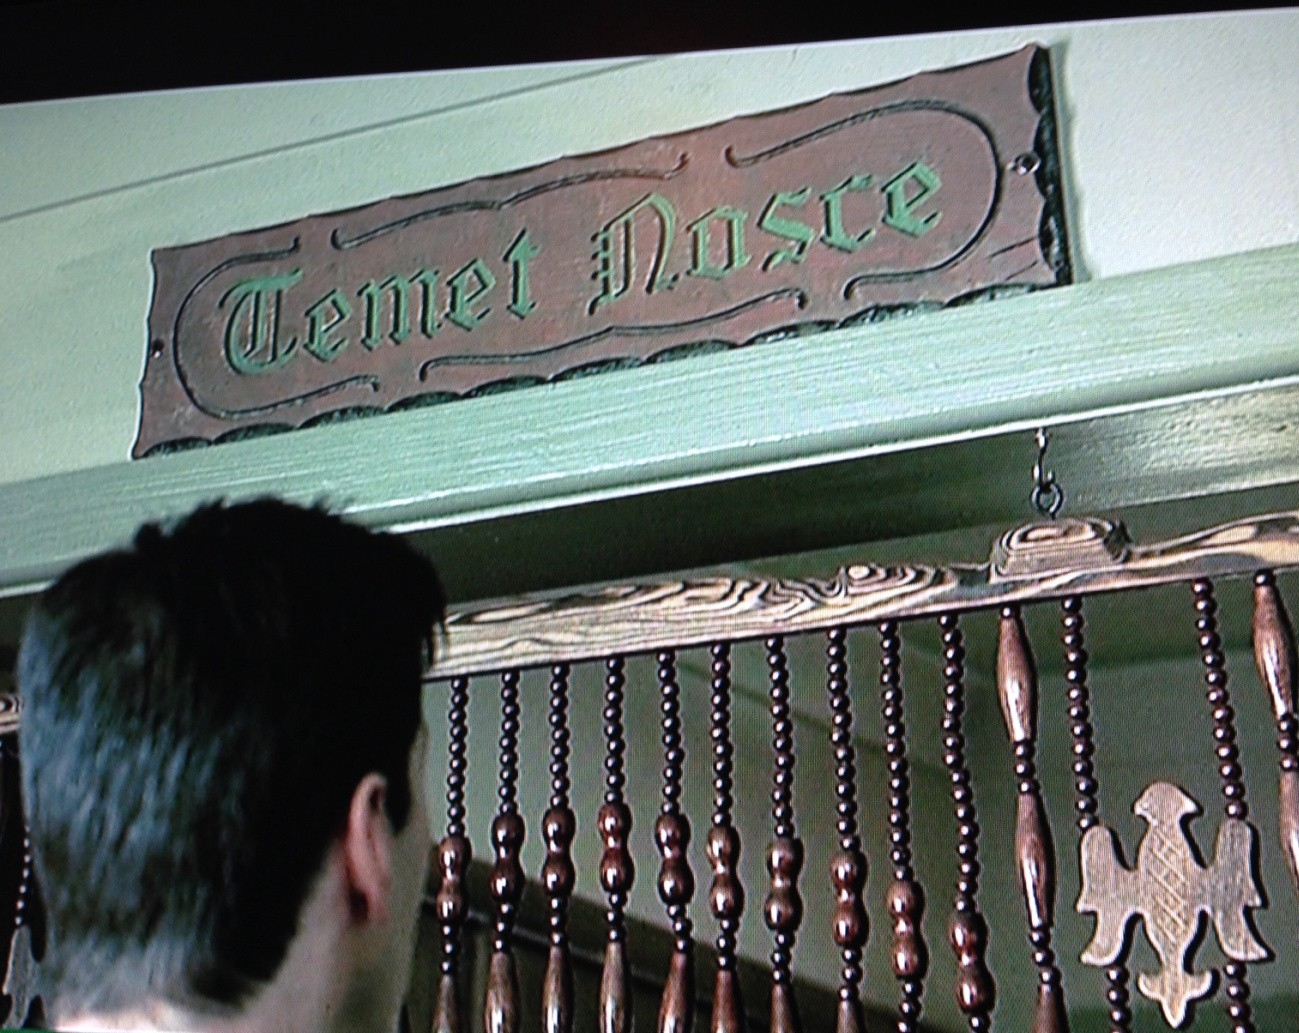
\includegraphics[width=6cm]{bilder/matrix.jpeg}
	\caption*{Begreppet ”känn dig själv” förekommer i många variationer, t.ex. i filmen The Matrix (1999).}
\end{wrapfigure}

Aforismen ifråga är dock äldre än de knappa trehundra år emellan oss och upplysningens Sverige. Det är uppenbart att aforismen var viktig även för antikens greker, då begreppet var inskrivet i väggen vid Apollons tempel i Delfi\footnote{Miller, J. Examined Lives: From Socrates to Nietzsche, 1. t., Farrar, Straus and Giroux 2011, s. 22}.

Den skarpa läsaren frågar sig varför detta är relevant för ett gulisnummer. Studenttidningar och dylika infoblad brukar innehålla en hel del goda råd åt de nya. Skaffa bostad, kom ihåg att delta i fritidsverksamheten, gnäll om pengar av FPA osv. Bland allt detta kan det vara svårt att komma med något revolutionerande och intressant. En svår målgrupp för skribenter, vilket i första hand beror på att de naturvetenskapliga gulisarna tenderar att vara oskulda. Alltså vad gäller studielivet. Det är krävande att förklara hur allt fungerar, lite som att förklara åt ordningsvakten att nej, det var varken du eller din kompis som spydde i hörnsoffan. Kemister destillerar olika saker med varierande framgång och här följer mitt försök att destillera en gnutta sanning.

Sun Zi, en kinesisk general född ca 500 f.Kr., skrev klassikern Krigskonsten. I detta epos konstaterar han att ifall man känner sig själv och fienden, behöver man inte frukta resultatet av hundra strider\footnote{Sawyer, R.D. The Seven Military Classics of Ancient China, Basic Books, 2007, s. 421 – 422}. Men vem är fienden? Det kan vara FPA med deras inkomstgränser från helvetets åttonde krets eller kanske ens egen lathet inför tenten. Faktum är att motståndarna är många och av varierande form, men självkännedom om ens styrkor och svagheter är konstant.

Och här kommer vi tillbaka till att känna sig själv, då det kan vara svårt att veta vad man vill. Studielivet är dock en utmärkt chans att vidga sina vyer. Många lär sig sina fysiska gränser på festernas sena timmar. Andra lär sig mentala dygder, såsom tålamod, genom sin första styrelsepost (det bör påpekas att det som händer i styrelsen stannar i styrelsen). Detta för att nämna några exempel.

Risken finns att självkännedom är ett fenomen av zenbuddistisk kaliber. Man kan inte bli upplyst om man ämnar bli upplyst, utan man måste snubbla på sanningen av misstag. Inte så långt ifrån att snubbla på tamburmattan i morgonmörkret.

Men hur borde man gå till väga? Det finns knappast ett definitivt svar. Mitt råd lyder att pröva olika saker, även om man tvekar, t.ex. tidigare nämnda styrelseposten. Av erfarenhet är det känt att ofta blir man positivt överraskad. Olika upplevelser avslöjar nya sidor av ens karaktär. Besök även andra föreningar, där man med god sannolikhet lär känna färggranna personer. Ofta har de annan inställning än en själv till flera frågor, vilket i bästa fall leder till ögonöppnande aha! -upplevelser. Även Paul Bragiel, VD för i/o Ventures, ett av de största investeringsbolagen i Silicon Valley, konstaterade att det bästa med universitet är att träffa spännande personer.

Spektrum är en liten men hårt sammansvetsad förening, vilket gör det enkelt att lära känna de andra. I mitt tycke är det också ett utmärkt sätt att utmana sig själv och knyta nya vänskapsband. Alla är välkomna att delta i verksamheten, även om de inte ämnar fortsätta studera naturvetenskaper. Några av er kommer att hitta er plats i livet på något annat ställe. För er vill jag citera Marcus Aurelius (1 21 – 1 80 e.Kr.), romersk kejsare och en av de få män som uppfyller Platons utopistiska vision om en filosof som kung\footnote{Aurelius, M. Meditations: A New Translation, övers. Hays, G., Modern Library, 2002, s. i}: 

Även om du gett upp hoppet om att bli en stor tänkare eller vetenskapsman, ge inte upp hoppet om att uppnå frihet (7.67)

\end{artikel}

\begin{artikel}{Medlemspresentation}{}

\textit{Eftersom det är mycket nytt när man är gulis, så tänkte vi att det kunde vara bra med en presentation av aktiva medlemmar som på ett eller annat sätt utmärker sig. Detta är alltså inte alla Spektrums medlemmar! Vi bad helt enkelt Spektrums medlemmar att skicka in en kort textsnutt om andra medlemmar och här är nu en sammanställning av dem. Förhoppningsvis gör presentationerna det lättare att lära känna och känna igen spektrumiterna. Om inte, så känns de igen på att de i princip är de enda som talar svenska uppe i Gumtäkt...}

\begin{twocolumns}

%Man är antingen andra årets kemist/fysiker/whatever eller sen nämner man inte månte året (gamyler kanske exception)
%Styssemedlemmar samt idrotts-, kafferums- och ADB-ansvarigas poster bör nämnas. PRK, värdar etc. behöver inte nämnas.
%Då sparar man uppdatering och huvudvärk :)

%Om ingen i redaktionen känner individen skall man fråga sig om individen i fråga har varit någo aktiv. Om jo, fråga andra spektrumiter för att hjälpa till med presentationen.

%Håll presentationerna ett år (RGL medlemmar två år) efter att hen har blivit inaktiv. Ibland kommer de också tillbaka! Tillsätt en "ta bort 20XX" kommentar på sådana

\textbf{Alvar} - Ekonometriker vars närvaro vid föreläsningar är godtyckligt nära noll. %ta bort 2021

\textbf{Amanda O} - F.d. föreningens sekreterare som böt från kemma till mattalärarlinjen. Har en inbyggd promillemätare. %ta bort 2021

\textbf{Amanda P} - En av de sällsynta statistikerna. Musikälskare som drömmer om att bilda en kör inom Spektrum. %ta bort 2021

\textbf{Anders} - Aktiv ekonometriker och Spektrums skattmästare som ofta hörs försöka påbörja Bang! i kafferummet. Alternativt hittas han ofta på Unicafe, var han äter i princip alla dagens måltider.

\textbf{Andreas} - Alltid lika positiv fysikstuderande som just nu utför sin värnplikt i Finlands djupa skogar.

\textbf{Anna} - Glad andra årets kemist som ofta syns till i Kafferummet och på Klubben. Miljö- och kulturansvarig.

\textbf{Anton} - Andra årets datavetartrumpetistesbobotutor. Del av soon-to-be-infamous Lärkangäng.

\textbf{Aslak} - Spektrums egna lapplänning som spenderar misstänksamt mycket tid till sjöss. Studerar fysik, är en av Spektrums trakasseriombudsmän och är grundaren av Spektrums bokklubb. Medlem i suprekordlaget Mys Mys.

\textbf{Chloé} - Fysikstuderande och en av Spektrums tutorer. Man kan samla pluspoäng med henne om man har en iphoneladdare att låna.

\textbf{Dan} - En professionell datalog som har de bästa algoritmerna och ett maffigt skägg. %ta bort 2021

\textbf{Daniel} - Data fysiker hybrid. Spektrum appens och Discord-bottens kodare. Medlem i suprekordlaget Mys Mys.

\textbf{Dennis} - Ett geni som har kommit längre i matematikssstudierna än sin tutors tutor.

\textbf{Emil A} - Statistiker och tutor som gärna spelar brädspel och kläcker ur sig några dank memes nu och då i kafferummet. Har den absolut viktigaste posten: Programchef.

\textbf{Emil L} - Invandrade från Lancaster en dag och har sedan dess ofta setts i kafferummet, våndandes över sitt jobb på acceleratorlabbet.

\textbf{Emma} - Glad och rolig geograf som once in a blue moon vågar sig till kafferummet. Ses främst på Spektrums sitzer och andra evenemang. Fungerar som tutor och Spektrums studiesekreterare.

\textbf{Eva} - Kemist som vet hur man festar. Om du känner att du saknar ett par till beer pong eller någon att shotta med så är Eva your girl.

\textbf{Frans} - Fysiker som alltid uppskattar en god whiskey. Även känd som ``Herra Isoherra'', och för att ha varit den officiellt kompaktaste ordföranden inom Spektrum. \emph{RGL}

\textbf{Gabriella} - Born and raised in Replot, Pampas. En ''priima'' andra årets fysiker javisst, men var studerar hon? Jämställdhetsansvarig.

\textbf{Henrik} - Stolt pampes och smart kemist. Kallas ibland vid namnet “Stubb”, som emellanåt sjungs entusiastiskt på sitzer och ingen vet riktigt varför... %ta bort 2021

\textbf{Hugo} - Sportig kemist och som är aktiv på många håll inom föreningen, t.ex. med att vara Spektrums ordförande. Spektrums Dressmann modell.

\textbf{Ida} - Medlem i den allt växande Ekenäsklubben. F.d. mattatutor. %ta bort 2021

\textbf{Iiro} - Lidande Lojobo som främst är aktivt med på TvEx-evenemang och i kemisternas ämnesförening. Mörkö. %ta bort 2021

\textbf{Inka} - Andra årets kemist som är en stamkund på Klustret. En bättre beer pong spelare är svår att hitta, trots detta klarar hon inte riktigt av att vinna en mot tre. %ta bort 2021

\textbf{Jeremias} - Lång matematiker som beslöt sig för att bli doktor i datavetenskap. Klättrar och spelar bridge med nylänningar. \emph{RGL}

\textbf{Jim} - En rojsig andra årets kemist från Borgå som tacklar folk i fritiden.

\textbf{Julia} - Trevlig och ärlig andra årets kemist från Sibbo som tror sig vara mer awkward än vad hon egentligen är. Gillar heart-to-heart diskussioner.

\textbf{Kalle} - Fysiker, hobbyfilosof, nuvarande sekreterare och f.d. tutor. Gillar musikalen Hamilton, anime och är en aktiv deltagare i Spektrums bokklubb.

\textbf{Mackan} - En härjande legend och på kommande. Spektrums jazz-hipster som hummar eller trummar alltid på nåt. Studerar matematik.

\textbf{Markus} - Datavetare samt ADB-ansvarig från Sibbo som hajoo med kandi. Officiell medlem på Spektrums inofficiella go klubb.

\textbf{Mats} -  Chill matematiker vars namn man alltför ofta glömmer. Löser världens problem ett i taget. %ta bort 2021

\textbf{Meri} - TvEx-kemist och f.d. Sveaborgfånge som alltid uppskattar finska ordvitsar. Har flest Jukola- och Venla-starter i Spektrums namn.

\textbf{Micaela} - Aktiv och glad andra årets fysiker. Kan verka ofarlig, men låt inte skenet bedra eftersom hon lär kunna en hel del om kampsport. En av två trakasseriombudsmän.

\textbf{Michaela} - Andra årets geograf som gillar att hitta på kortspel. Syns alltid då och då på evenemang.

\textbf{Moonika} - Tvexande kemist från Uleåborg. Är aktiv i både HYK och Spektrum, och råkar även vara en väldigt tävlingssinnad beerpongspelare. %ta bort 2021

\textbf{Oliver} - En äkta fysikergamyl som alltid syns till på Klubben då det händer något. Trösklar är hans överraskande fiende, öl ej!

\textbf{Oskar Bj} - Matematiker, datalog och allvetargamyl. Gillar Rudin, Clojure och abstraktion. %ta bort 2021

\textbf{Oskar Br} - Matematiker. Syns i kafferummet eller på Spektrums sportevenemang, som han ordnar då och då.

\textbf{Oskar F} -  Kapabel matematiker, de flesta känner honom som ``Åland''. Vet mycket om drycker, både som klubbmästare och som förbrukare. Medlem i suprekordlaget Mys Mys.

\textbf{Otto} - En realist från Sibbo som alltid är redo att hjälpa föreningen och får saker gjort. Har den största namnskylten på Klubben. \emph{RGL}

\textbf{Philip} - En filosoferande datalog som vill lära sig om allt. Har utfört diplomatiskt arbete i Arabien. %ta bort 2021

\textbf{Rasmus N} - Även kallad Nisse är fysiker och f.d. tutor. Aktiv pünchenhävare som inte behöver mer än en flaska Leijona för att underhålla sig i flera timmar. Kafferumsansvarig.

\textbf{Rasmus T} - Andra årets matematiker/datavetare som hittas i Exactums tredje våning kämpandes med epislon-delta bevis eller något annat lika ``kul''. %ta bort?

\textbf{Robert Ho} - Glad och chill datalog och ADB-ansvarig. Kan alla de bästa babyskämten.

\textbf{Robert Hä} - Nördig matematiker som flydde till Innsbruck, Österrike föregående läsår. Fick nog av joddlande och beslöt sig att returnera till Finland.

\textbf{Robert P} - Ex-fysiker som gjorde ett bra beslut och migrerade till datavetanskap. Tennisproffs. %ta bort 2021

\textbf{Robin} - Trevlig, dataspelande fysikstruderande som härstammar från Veikkola. Tydligen hade suttit med i styrelsen förra året? Spektrums Go master. %ta bort 2021

\textbf{Sami} - Fysiker som enligt gumtäktska folksagor är snabbare än ljuset. Detta brukar inte hindra honom från att njuta av en extra akademisk kvart då och då. %ta bort 2021

\textbf{Sara} - Datav... korjaus: matematiker som fungerar som föreningens viceordförande. Hittas ofta i kafferummet spelande diverse kortspel eller på sitzer i vilka hon \emph{aldrig någonsin} svinar. Spektrums största svamlare.

\textbf{Sebastian ``Sebbe'' H} - Sportig fysiker från Österbotten. Spektrums mångårige Jukola-ansvarige som nu även ibland kan hittas högst upp i Physicum. Chefredaktör (som ni redan visste, eller hur?)

\textbf{Simon} - En allt för ärlig matematiklärarstuderande som vet hur man njuter av livet. Golfar med bollar och frisbees. ’Nuff said.

\textbf{Sonja} - En musikalisk matematiker som spelar violin och sjunger i kör. Inte en rysk specialagent. %ta bort 2021?

\textbf{Stefan} - Spektrums största och hårigaste ålänning. Gillar öl, whisky och metal. %ta bort 2021?

\textbf{Tobias} - Åbokemist i början, nuförtiden huvudstadsbo. Går med stil, oberoende hur hett det är. Kan ses på Klubben lite nu som då. %ta bort 2021?

\textbf{Toffe H} - Andraårsfysiker med en killer smile. I hans egna ord: sheltered white boy. Panini 4 life.

\textbf{Toffe F} - Hör till den alltid lika soliga Spektrala Pampasligan. Kan hittas i acclabbet eller i kafferummet. Visar närpå omänskliga kunskaper då någon har problem med datorn. \emph{RGL}

\textbf{Victor} - Svinande fysiker som gör allt enligt sitt eget tempo, dock ändå får saker gjort. Då någon säger ansvar, vänder Victor andra kinden till. Kafferumsansvarig... kanske?

\textbf{Viktor ``Horsmanheimo'' Horsmanheimo} - Datavetare vars närvaro i Exactum och sitzer inte går att missa. Njöt av värnplikten och njuter ännu mera av kryssningar.

\textbf{Viktoria ``Titti''} - Matematiker, trots att hon nästan valde kort matematik i gymnasiet. Titti går på sushi och aperol, och är f.d. tutor.

\textbf{Waffe} - Kodar eget programmeringsspråk varav ni kommer att höra nog. Spelproducent, rollspelare, animeabsorberare, redaktionschef och kaffegillare. Ger dig jobb som byktvättare.

\textbf{William} - Färsk kemist, hajo i milin och njuter nu av friheten. Syns i kafferummet alltid då och då.

\end{twocolumns}

\picture[]{bilder/rubber_sheet.png}[xkcd.com]
\end{artikel}

\begin{artikel}{Ett litet val i all hast - hur jag blev tvåspråkig}{Meri Sillanpää}[]
\begin{twocolumns}

\textit{Ensimmäinen yliopistopäiväni kolme vuotta sitten. Keskustassa aamulla ruuhkaa ja olen myöhässä vartin. Integraalimäestä hengästyneenä ja hivenen hikisenä saavun vihdoin Chemicumin aulaan. Aula on lähes tyhjä, muutama tuutori istuu pöydän ääressä ja ennen kun he neuvovat minut oikeaan luentosaliin, saan pienen paperilapun täytettäväksi.}
 
\vspace{0.2cm}
\noindent\fbox{%
    \parbox{\linewidth}{%
        \vspace{0.1cm}
        Nimi:
        
        Olen kiinnostunut:
        
        $\square$ Ope-opinnoista
        %\mbox{\ooalign{$\checkmark$\cr\hidewidth$\square$\hidewidth\cr}}
        
        $\square$ Kaksikielisestä tutkinnosta
         \vspace{0.2cm}
    }%
}
\vspace{0.2cm}

% holla holla get dolla
% check the check you speck of fläck
% Tanken var att dedär e lappen hon fick framför sig
% Såhär
% Dedär va good idea of you, thanks

Nimi? Helppo homma. Kiinnostuksen kohde oli sen sijaan kiireessä hieman vaikeampi kysymys. Tiesin etten halua opettajaksi, sen sijaan en ollut koskaan kuullutkaan kaksikielisestä tutkinnosta. Muistan edelleen mitä ajattelin seistessäni lappu kädessä keskellä aulaa, myöhässä ensimmäiseltä orientaatio luennolta: ”Voihan siitä olla kiinnostunut, ei se tarkoita että tutkintoa tarvitsisi tehdä kaksikielisesti”. Joten myöhässä ja kiireessä rastitin ruudun ”kaksikielinen tutkinto”, annoin lapun takaisin tuutorille ja kiiruhdin luennolle.

\columnbreak
Utöver detta kommer jag inte ihåg mycket mera av min första dag vid Uni, men jag kommer ihåg detta lilla val som gjordes i all brådska för det har påverkat mycket mitt studieliv. Tack vare den tvåspråkiga examen (TvEx) kom jag också med i ämnesföreningen Spektrum, som är en ypperlig plats för att utforska studielivets bästa sidor; fest, Klubben, sits, nya vänner och förstås billiga drycker. Att öva samt lära sig ett nytt språk lyckades ganska naturligt sådär samtidigt. När man börjar på TvEx-programmet förväntar sig ingen att du skulle kunna det andra språket perfekt, det enda som krävs är motivation och vilja att lära sig. I Spektrum kritiserar man inte språkfel, utan man uppmuntrar andra för att försöka deras bästa. Man skulle kunna säga att det finns en oskriven regel inom Spektrum: Om du vill, så får du alltid prata ditt eget modersmål, oberoende om det är finska eller svenska.

Itselle ehdottomasti paras tapa oppia uutta kieltä oli kuunnella ja käyttää sitä. Olkaa siis itse aktiivisia, ennakkoluulottomia ja osallistukaa myös vieraskielisiin tapahtumiin. Mutta ennen kaikkea, nauttikaa kaikista niistä kokemuksista, joita tuleva (mahdollisesti kaksikielinen) vuosi voi teille tarjota.

\end{twocolumns}
\end{artikel}

\newpage

\begin{artikel}{Presentation av ämnesföreningar}{}

\textit{Som kanske inte så många av er vet så finns det fler ämnesföreningar inom Gumtäkts
väggar. Spektrum är den enda helt svenskspråkiga, men finskspråkiga finns fler än väntat. Så
om man vill finslipa det andra inhemska språket lite så talar de finskspråkiga studerandena
mer än gärna med en. Här har en del av de finskspråkiga föreningarna skrivit en liten
presentation om deras förening, på svenska! Ta er en titt, så finner ni kanske en ny
vänförening.}

\textbf{Limes}

Limes är en ämnesförening från Gumtäkt som grundades redan 1 936.
Om du studerar vad som helst i Gumtäkt är Limes din förening. ;)
Vi organiserar olika evenemang - från bastukvällar och exkursioner till sitsar och bileen.
För oss är det största evenemanget Limeksen Appro, som årligen får 2000-3000 deltagare.
Vi säljer också läroböcker och halarmärken förmånligt.
Välkommen att bli medlem vid vårt kontor som ligger i Exactum, rummet C132! <3
(Genast brevid kafferummet -chefr)

\textbf{HYK}

Helsingin Yliopiston Kemistit ry eller HYK är den finskpråkiga ämnesföreningen för kemister i Gumtäckt.
HYK är grundad år 1 927 och är en av de äldsta studentförenringar i Helsingfors
Universitet.
Vi älskar traditioner men också att oganisera nya händelser för våra medlemmar.
Man hittar kemister i svarta overaller i Opsos, HYKs kafferum, som ligger i Chemicum.
Välkommen!

\textbf{Geysir rf}

Geysir rf grundades år 1 997 och är blivande geofysikers intresseorganisation. Vårt mål är att ordna en så mångsidig underhållning som möjligt för våra medlemmar: exkursioner,
dvs studiebesök hos studie- och forskningsanstalter samt på isbrytare och på havsforskningsfarty, idrott (bl. a. väggklättring), kultur (filmer, teater, konserter) samt soaréer (film- och spelkvällar). Exkursionerna till utlandet ingår sedan länge i Geysirs traditioner. Sådana besök inträffar vanligtvis med två års mellanrum. Vi har nyss varit på Island, vid Spetsbergen, på Azorerna, på Nya Zeeland och i Etiopien. Målet för resan år 2014 var Ungern, och var och en är välkommen att komma med idéer till vår nästa resa för år 2016!

\textbf{Synop ry}

Synop ry är meteorologiska ämnesorganisationen som har hjälpt människor rikta sina
ögon mot moln för redan 45 år. Vi är ganska liten, men aktiv organisation som ordnar olika
slags evenemang från sport och filmkvällar till bingor. Den största bingon ordnas varje vapp
och alla är välkomna. Mer information om oss kan ni hitta från vår webbsida www.atm.helsinki.fi/synop eller studentrumet i Physicum där det ofta finns några medlemmar.

\textbf{Meridian rf}
Tycker du om att vara vaken helan natten och att sova hela dagen? Meridian rf
(Meridiaani) är en ämnesförening för astronomistudenter i Helsingfors universitet. På hösten
har vi olika slags evenemang för unga astronomer, vi grillar, spelar brädspel och vår ölklubb träffas varje månad. På våren organiserar vi ett berömd rymdparti Yuri's Night. För att observera stjärnor, planeter och galaxer användar vi en 60-cm teleskop i Metsähovi
Obsevatoriet i Kyrkslätt. Du kan hitta oss i Gumtäkt i Physicum's Studentrummet OH med de
andra fysikerorganisationerna.

\end{artikel}

\begin{artikel}{Byggnader i Gumtäkt}{Sandra m. fl.}

\textit{Hej alla nya studeranden och även ni lite äldre. Här kommer en liten presentation över byggnaderna som finns vid Gumtäkts campus. Så om ni aldrig har varit där tidigare,
eller inte tillbringat tid där på så länge att ni inte minns hur det ser ut mera, så kan
det vara en bra idé att ta er en titt på denna artikel.}

\picture[width=12cm]{bilder/chemicum.jpg}

\textbf{Chemicum}

Kemiströvarnas härbärge. Byggnaden är åtskild från de övriga, vilket brukar resultera i att endast kemister rör sig i ”Chemen”. Om vi andra studeranden drar oss ditåt är det för det mesta för att stilla hungern i matsalen. Svenska chemen fanns tidigare i denna byggnad, men tyvärr har vi fått säga adjö till detta svenskspråkiga fenomen. Spektrums kafferum brukade vara i Chemicum, förrän alla matematiker började gnälla om den långa vägen dit.

\picture[width=12cm]{bilder/Exaktum.jpg}

\textbf{Exactum}

Det är här alla matematikrumpnissar och datalogvildvittror håller hus. Den ökända Integralbacken (d.v.s. Djävulsbacken) leder upp till denna byggnad, och är orsaken för flera förseningar och diverse mindre skador. Datalogerna befinner sig oftasts på andra våningen eller i källarvåningen, medan matematikerna håller hus på tredje våningen. På tredje våningen finns även en mängd allmänna brädspel, som schack och go. I Exactums första våning ligger både Linus Torvalds auditorium och Lars Ahlfors auditorium, där de flesta tenterna skrivs. Utöver detta finns Spektrums kafferum i Exaktum, där alla flitiga och mindre flitiga spektrumiter håller hus.

\picture[width=12cm]{bilder/Physicum.jpg}

\textbf{Physicum}

Här styr och ställer grådvärgsfysikerna. Ska man till Physicum brukar oftast den högra delen av djävulsbacken vara den rätta vägen att ta. I Physicum finns det både det ena och det andra. Biblioteket, där man förvånansvärt nog kan låna böcker eller bara sitta och studera ostört, samt ett café, där det säljs paninin, baguetter (eller ``patonkin'', som de i folkmun också kallas) och goda bullar. ”Sandlådan” är också ett ställe där flitiga studeranden kan samlas; denna del finns på högsta våningen i Physicum. Det finns självfallet också utrymme för klassrum. I dessa klassrum finns både fysiker, geologer och andra fysikintresserade människor.

Från och med 2018 delades fysikavdelningen vid Helsingfors Universitet in i två delar: en för det mesta oförändrad, “allmän” fysikavdelning och till Institute for Atmospheric and Earth System Research (INAR), som är en forsknings- och undervisningsavdelning inom atmosfärvetenskap. I Physicum hittas även HIP- Helsinki Institute of Physics.

På Physicums andra våning finns även kansliet, dit ni borde gå för att bland annat få ett fint klistermärke på ert studiekort. Om man har andra frågor är det också dit man borde röra sig. 

\picture[width=12cm]{bilder/Labbet.jpg}

\textbf{Acceleratorlabbet}

Acceleratorlabbet är stället alla viktiga fysiker samlas på. Vem de är och vad de gör där vet ingen, men rykten går kring Gumtäkt som en löpeld.

Förutom dessa finns Dynamicum, där de icke-Astrid Lindgren-relaterade meteorologiforskarna befinner sig; samt Unisport, dit alla sportiga och ibland icke-sportiga rör sig för att röra på fläsket.

\end{artikel}

\begin{artikel}{Haikun: Veckoslut}{}
En diktsamling av pseudo-moderna haikun av den snart världsberömda, dock alltid söndriga, yrbollspoeten Emil L.
\vspace{0.5cm}

\textbf{Förord}

Min kära Jonas.\\
Du sade: EN artikel.\\
Min förrädare.


\vspace{0.8cm}

\textbf{Bok 1: Att vaka}

\begin{flushleft}
Skrivit på kandin.\\
Hela dagen i Gumtäkt.\\
Dags att gå sitsa.
\end{flushleft}

\begin{center}
Alla sätter sig.\\
Nu äter vi och sjunger;\\
med snaps, efter snaps.
\end{center}

\begin{flushright}
Helan och halvan,\\
och någonting om minnet.\\
Nej! Int Theobald...
\end{flushright}

\begin{flushleft}
Nu kommer punschen.\\
Usch vad jag hatar punschen.\\
Men dricker ändå.
\end{flushleft}

\begin{center}
Nån spelar beerpong.\\
Hen kastar bollen, missar.\\
Bollen hittas ej.
\end{center}

\begin{flushright}
Sen sade Herr J:\\
``Ditt hår luktar till anus''\\
Gjorde mig ordlös.
\end{flushright}

\begin{flushleft}
Herr V drack en öl.\\
Han skrattade, men varför?\\
Han är i fyllan.
\end{flushleft}

\begin{center}
En shot, två shot, tre.\\
Jag är bäst på att dansa.\\
Fyr shot, fem shot, spy.
\end{center}

\begin{flushright}
``Det är dags att gå.''\\
Tre timmar senare dock,\\
är det dags att gå.
\end{flushright}

\begin{flushleft}
Oändlig hunger.\\
Jag skådar en snägäre.\\
``Ge mig en lihis.''
\end{flushleft}

\begin{center}
Äntligen hemma.\\
Jag törstar, öppnar kylen,\\
ser en gatorade.
\end{center}

\vspace{0.8cm}

\textbf{Bok 2: Att vakna}

\begin{flushleft}
Jag drömde om Fymm\\
och vaknade till Kvant. Mek.\\
Vill ej leva mer.
\end{flushleft}

\begin{center}
Ack, vilken fiilis.\\
Ack, var äro ämbaret?\\
Ack, det är för sent.
\end{center}

\begin{flushright}
Ett steg från sängen.\\
Men hela världen snurrar.\\
Lägger mig igen.
\end{flushright}

\begin{flushleft}
Mitt huvve bultar.\\
Det finns ingen burana.\\
Är detta slutet?
\end{flushleft}

\begin{center}
Torr som sahara.\\
Långsam som en sköldpadda.\\
Sätter på Netflix.
\end{center}

\begin{flushright}
Tar fram snapsboken,\\
Läser allas små skrifter.\\
Så många kukar.
\end{flushright}

\begin{flushleft}
Vad strupen törstar.\\
Var äro min gatorade?\\
Nån har druckit den.
\end{flushleft}

\begin{center}
Kokade kaffe.\\
Njuter av svarta guldet.\\
Måste på vessa.
\end{center}

\begin{flushright}
Det värsta är slut.\\
Min mage börjar kurra.\\
Ser en halv lihis.
\end{flushright}

\begin{flushleft}
Tröttheten stiger.\\
Inspirationen lider.\\
Kan ej skriva mer.
\end{flushleft}

\begin{flushright}
\emph{Emil L. - söndrig poet och allmän yrboll}
\end{flushright}

\vspace{1.6cm}
\picture[]{bilder/phdf.jpg}

\end{artikel}


%----------------------------------------------------------------------
%	This command prints the publisher information on one line with
%	all fields separated by 'bullets'.
%----------------------------------------------------------------------
\lastpage{0.9\textwidth}{bilder/RELEX_A5.pdf}

\end{document}